\section{High Performance Computing}
\label{sec:CDA_HPC}

\gls{HPC} has been an integral part of scientific research and engineering for decades.
While it is being used synonymously with supercomputing\footcite{sterlingHighPerformanceComputing2017},
the term \ac{HPC} is used to describe the use of supercomputers and parallel processing techniques for solving complex computational problems that respond to scale, meaning that the application of more resources will result in a more valuable product.

\ac{HPC} systems are designed to go beyond the capabilities a single system can provide,
and therefore utilizes clusters of multiple computers that work together to solve a problem instead.
% Note from Harumi: I took out the "not just" because there was no matching "but also"
% Note from Harumi: Also, I merged in the following paragraph because it was a single-sentence paragraph
These systems have enabled scientific breakthroughs,
like the research on the human genome\footcite{schadtComputationalSolutionsLargescale2010},
the discovery of the Higgs boson\footcite{belyaevHighPerformanceComputing2017} or the first image of a black hole\footcite{hlrshighperformancecomputingcenterstuttgartHLRSHighPerformance}.
That said, \ac{HPC} systems are by no means limited to purely scientific applications,
as they are also an essential tool in various industries, such as finance, oil and gas, automotive, and many more which
require complex simulations, data analysis, and modeling\footcite{fortunebusinessinsightsHighPerformanceComputing}.

% Note from Harumi: I suggest a rewording here because I think CC systems have also been around for
% decades. It's just that they have only recently begun to feature HPC-scale workloads.
Supercomputers, which have been around for many decades, have historically focused on how to scale performance so as to produce more valuable results by applying more computing resources.
For this, \ac{HPC} systems sacrifice ease-of-use in favor of performance, employing \gls{bare metal} systems and highly specialized homogeneous hardware.  \ac{CC} systems,
however, have only recently begun to take on \ac{HPC}-scale workloads.
\ac{CC} systems are tailored to maximize ease-of-use, and have historically sacrificed performance for the sake of offering increased flexibility and reliability.
As \ac{AI} workloads have increased in size, the task of managing \ac{HPC} clusters has become more expensive and complex.
With cluster sizes increasing to thousands of nodes, the two communities have been moving towards each other.
That is to say, \ac{HPC} customers have become increasingly interested in ease-of-use and \ac{CC} customers have become increasingly interested in performance-at-scale.

\subsection{Introduction to High Performance Computing}

At its core, \ac{HPC} revolves about the concepts of distribution and parallelization -- the spreading of highly complex computational tasks across multiple systems
to solve problems that are too large or too complex for a single computer to handle.
Therefore, its main issue is the splitting of a problem into smaller tasks that can be solved in parallel, as well as the coordination of running separate nodes as to work together in a coordinated manner.

\ac{HPC} differentiates between two types of compute problems:

First are the so-called \textit{embarrassingly parallel} problems, which are sometimes also referred to as \textit{pleasingly parallel} problems.
Such problems have gotten their name by the ease of parallelization, as they can be split into independent tasks that can be solved in parallel.
Classical examples include the Ray tracing of images, where each pixel can be calculated independently,
or Monte Carlo simulations\footcite{gandyAdvancedComputationalMethods}.

In contrast to that is the true challenge of \ac{HPC} -- \textit{strongly coupled} problems,
where the different tasks are dependent on each other and therefore need to be solved in a coordinated manner.
Classic examples of this include weather simulations, \texttt{Finite Element Analysis} or \texttt{n-body} simulations\footcite{capuzzo-dolcettaFullyParallelHigh2013}.
As each element of the simulation is highly dependent on all or at least a subset of the other elements,
a high need for inter-node-communication arises.

% Therefore, the second most important part of a \ac{HPC} system after the compute nodes themselves is the interconnect,
% which is responsible for communication (especially, data exchange) between the nodes. 
% This can be seen  in the \ac{HPC} Top500 list, where the fastest supercomputers are ranked by their \texttt{LINPACK} performance,
% which measures the speed of solving a dense system of linear equations\footcite{dongarraLINPACKBenchmarkPresent2003}.
Therefore the two  most important parts of a \ac{HPC} system are the compute power of a given node on the one hand and the interconnect on the other.
This can be seen in how these systems are ranked in practice as the authority on \ac{HPC} performance, the \textit{Top500} list ranks the fastest supercomputers by their \texttt{LINPACK} performance,
which measures the speed of solving a dense system of linear equations\footcite{dongarraLINPACKBenchmarkPresent2003}.
As the \texttt{LINPACK} benchmark is a highly parallelize problem, the ranking is highly biased towards the raw compute power of the system,
as the communication need between the nodes is negligible.
In order to supplement this, the \texttt{Graph500} list was created, which ranks the systems by their ability to solve the traversal of a graph\footcite{murphyIntroducingGraph5002010}.
This provides an insight into the performance of a system when solving a problem that is not just a sum of the individual compute power of the nodes,
but is also highly dependent on the interconnects and the communication between the nodes.

\subsection{HPC Infrastructure}
\label{sec:hpc_infrastructure}

The core component of a \ac{HPC} system are the compute nodes, which are the individual systems that perform the calculations.
These nodes may be equipped with multiple processors, including \ac{CPU}s, \ac{GPU}s, or \gls{FPGA}s, and are connected to each other via a high-speed network.
While homogeneous systems only utilizing a single type of processor across all nodes are still common, a trend towards \ac{GPU} coprocessor systems can be observed\footcite{kindratenkoTrendsHighPerformanceComputing2011}.

In the past, the larger architecture of \ac{HPC} systems used to be much more diverse, employing architectures such as
constellations, \ac{SIMD}, or even single processor systems\footcite{top500ListStatisticsArchitecturea},
but more recently
\ac{MPP} and Cluster systems have become dominant.

% \todo{[Note from Harumi: I don't understand what "make up for it in performance" means in the following sentence.]}
% Currently, Clusters are the most common, making up over 80\% of systems, with the \ac{MPP} make up for it in performance \footcite{top500ListStatisticsArchitecture}.
% Correction:
While clusters make up 80\% of all \textit{Top500} systems, when scaled for the total compute power per architecture,
\ac{MPP} systems make up 44\% of the total compute power of the \textit{Top500}\footcite{top500ListStatisticsArchitecture}.

There are significant differences between \ac{MPP} and Cluster systems with regard to how they are connected and how they communicate.
Clusters are based on a shared-nothing architecture, where each node has its own memory and communicates via
messages over a network connection.
In contrast, \ac{MPP} systems are based on a shared-memory architecture,
where all nodes share the same memory and can communicate via this shared memory\footcite{dongarraHIGHPERFORMANCECOMPUTINGCLUSTERS2005a}.
However the size of cores per node has increased, these distinctions have become less pronounced.
% \todo{[Note from Harumi: I did not understand the following sentence and attempted to revise it.]}
This is because these multi-core systems also need to communicate internally, which may also be done via shared memory communication,
while communication between the nodes is still done via a network connection, creating a hybrid architecture\footcite{liNUMAawareSharedmemoryCollective}.

\subsubsection{Memory Architecture}

In a \ac{HPC} system the structure of the memory is one of the most distinguishing features of
the system, as it has a significant impact on the performance of the system, how it needs to
be programmed and what kind of workloads it is best suited for.

A significant difference between \ac{HPC} systems is how they manage the coordination between
the different compute cores. The two main architectures are either a shared memory based approach, generically
called \ac{SMP} which combines its parts into a single large operating system, enabling the processors
to access private, shared or common memory. The other approach is to have multiple separate systems,
keeping their memory exclusively to themselves, coordinating and sharing data through the passing of
messages over the underlying network or interconnect\footcite{archeruknationalsupercomputingserviceLectureHPCArchitectures2016}.


\textbf{UMA}

Its most basic implementation is a single node with multiple cores, where all cores have access to the same flat memory,
through a shared \gls{bus}, as can be seen in Figure~\ref{fig:smp}.
This is what is know as a \ac{UMA} system, where all memory is equally accessible to all cores.
Being able to access the same memory is a significant advantage of \ac{SMP} systems,
it is exceptionally well suited towards tightly coupled problems, where the different cores can directly
work on the same data, without the need to communicate over a network connection.
In the early days of \ac{HPC} this worked especially well, as \ac{CPU}s where much slower than
the memory itself.

\begin{figure}[!ht]
  \vspace{0.8cm}
  \centering
  \scalebox{0.8}{

    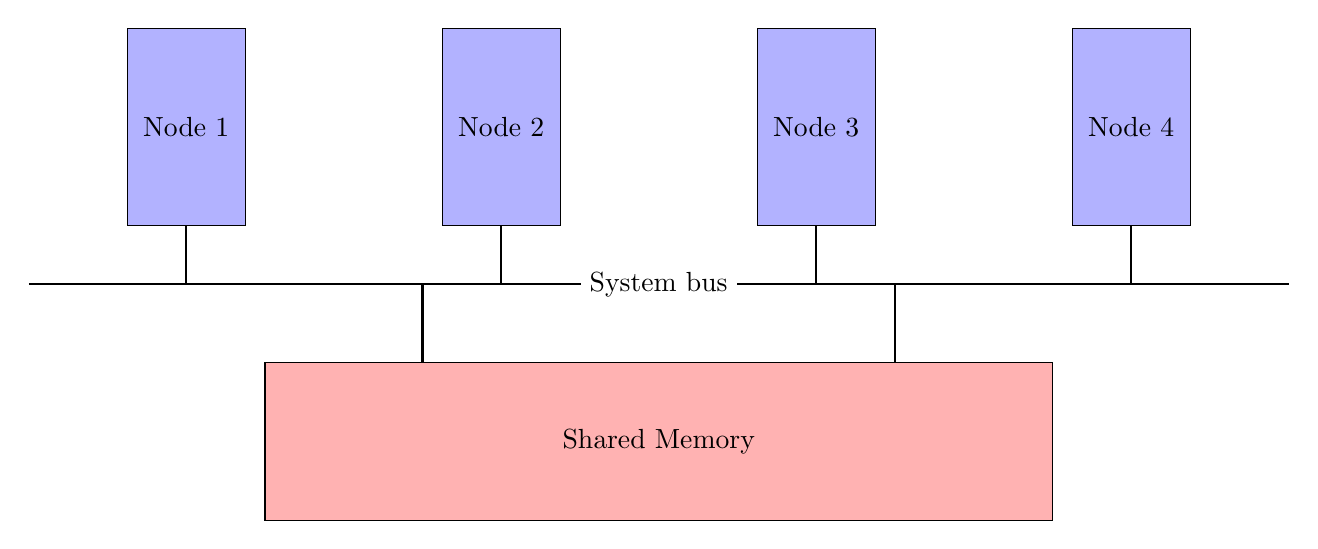
\begin{tikzpicture}
      % System \gls{bus}
      \draw[thick] (0,0) -- (16,0) node[pos=0.5, fill=white] {System bus};

      % Compute Nodes
      \foreach \x in {2, 6, 10, 14} {
          \node (CN\x) [draw, rectangle, minimum width=1.5cm, minimum height=2.5cm, fill=blue!30] at (\x, 2) {};
          \draw[thick] (\x,0) -- (CN\x);
        }

      % Labels for Compute Nodes
      \foreach \x [count=\xi] in {2, 6, 10, 14} {
          \node at (\x, 2) {Node \xi};
        }

      % Memory
      \node (MEM) [draw, rectangle, minimum width=10cm, minimum height=2cm, fill=red!30] at (8, -2) {Shared Memory};

      % Connections
      \foreach \x in {5,11} {
          \draw[thick] (\x,0) -- (\x,-1);
        }
    \end{tikzpicture}
  }
  \caption{Symmetric Multi-Processing (SMP) Architecture}
  \label{fig:smp}
\end{figure}

\ac{CPU} speed improvements outpacing memory technology led to the flat memory not being
able to keep up with the \ac{I/O} demand of the \ac{CPU}s; this problem has come to be commonly known as the \texttt{"von Neumann bottleneck"}.

\textbf{NUMA}

To alleviate this issue of the \texttt{"von Neumann bottleneck"} new, more distributed memory architectures have been developed.
The central idea is to create multiple smaller zones of collaboration  -- namely,
instead of having all cores having equal access to a single large chunk of memory,
allocating smaller chunks of memory to a few cores each which they can access quickly,
while still allowing them to access the memory of all other cores.
This prevents the issue of the \texttt{"von Neumann bottleneck"} by reducing the number of cores that need to access the same memory
while at the same time, but still allowing all cores to access the memory of all other cores.
This is what is called \ac{NUMA} architecture, as can be seen in Figure~\ref{fig:numa}.

\begin{figure}[!ht]
  \centering
  \vspace{0.5cm}
  \scalebox{0.9}{

    \begin{tikzpicture}

      % Nodes

      %node 1
      %CPU
      \node [draw, rectangle, minimum width=1cm, minimum height=1cm, fill=blue!30] (cpu11) at (-2, 2) {CPU1};
      \node [draw, below of=cpu11, rectangle, minimum width=1cm, minimum height=1cm, fill=blue!30] (cpu12) {CPU2};

      %Memory
      \node [draw, left=0.0cm of cpu11, rectangle, minimum width=2cm, minimum height=1cm, fill=red!30] (mem11) {Memory1};
      \node [draw, left=0.0cm of cpu12, rectangle, minimum width=2cm, minimum height=1cm, fill=red!30] (mem12) {Memory2};

      %Node box
      \node[draw,
        dashed,
        fit=(cpu11) (cpu12) (mem11) (mem12),
        inner sep=0.1cm,
        label={\scriptsize{Group 1}}
      ] (group1) {};

      %node 2

      %CPU
      \node [draw, rectangle, minimum width=1cm, minimum height=1cm, fill=blue!30] (cpu21) at (-2, -2) {CPU1};
      \node [draw, below of=cpu21, rectangle, minimum width=1cm, minimum height=1cm, fill=blue!30] (cpu22) {CPU2};

      %Memory
      \node [draw, left=0.0cm of cpu21, rectangle, minimum width=2cm, minimum height=1cm, fill=red!30] (mem21) {Memory1};
      \node [draw, left=0.0cm of cpu22, rectangle, minimum width=2cm, minimum height=1cm, fill=red!30] (mem22) {Memory2};

      %Node box
      \node[draw,
        dashed,
        fit=(cpu21) (cpu22) (mem21) (mem22),
        inner sep=0.1cm,
        label={\scriptsize{Group 2}}
      ] (group1) {};

      % node 3

      %CPU
      \node [draw, rectangle, minimum width=1cm, minimum height=1cm, fill=blue!30] (cpu31) at (2, 2) {CPU1};
      \node [draw, below of=cpu31, rectangle, minimum width=1cm, minimum height=1cm, fill=blue!30] (cpu32) {CPU2};

      %Memory
      \node [draw, right=0.0cm of cpu31, rectangle, minimum width=2cm, minimum height=1cm, fill=red!30] (mem31) {Memory1};
      \node [draw, right=0.0cm of cpu32, rectangle, minimum width=2cm, minimum height=1cm, fill=red!30] (mem32) {Memory2};

      %Node box
      \node[draw,
        dashed,
        fit=(cpu31) (cpu32) (mem31) (mem32),
        inner sep=0.1cm,
        label={\scriptsize{Group 3}}
      ] (group1) {};


      % node 4

      % CPU
      \node [draw, rectangle, minimum width=1cm, minimum height=1cm, fill=blue!30] (cpu41) at (2, -2) {CPU1};
      \node [draw, below of=cpu41, rectangle, minimum width=1cm, minimum height=1cm, fill=blue!30] (cpu42) {CPU2};

      %Memory

      \node [draw, right=0.0cm of cpu41, rectangle, minimum width=2cm, minimum height=1cm, fill=red!30] (mem41) {Memory1};
      \node [draw, right=0.0cm of cpu42, rectangle, minimum width=2cm, minimum height=1cm, fill=red!30] (mem42) {Memory2};

      %Node box
      \node[draw,
        dashed,
        fit=(cpu41) (cpu42) (mem41) (mem42),
        inner sep=0.1cm,
        label={\scriptsize{Group 4}}
      ] (group1) {};

      % interconnects

      \draw[thick] (cpu12) -- (cpu21);
      \draw[thick] (cpu11) -- (cpu31);
      \draw[thick] (cpu22) -- (cpu42);
      \draw[thick] (cpu32) -- (cpu41);

      \draw[thick] (cpu12) -- (cpu41);
      \draw[thick] (cpu32) -- (cpu21);


    \end{tikzpicture}
  }
  \caption{Three Tiered NUMA Architecture\protect\footnotemark}
  \label{fig:numa}
\end{figure}

\footnotetext{Diagram adapted from \cite{ploskasIntroduction2016}}

The diagram in \ref{fig:numa} shows a three-tiered \ac{NUMA} system, two processors having access to their own memory, while also being able to access the memory of the other processor.

\begin{enumerate}
  \item The \ac{CPU}s own cache which is the fastest to access.
  \item The cache of the \ac{CPU}s neighbor cores on the same group.
  \item The memory of the other groups.
\end{enumerate}

While this lets the \ac{SMP} systems scale much larger than the \ac{UMA} systems,
it also has to deal with the issue of keeping these distributed memory systems in sync,
as well as making sure to distribute this memory in a way that is optimal for the workload.


\textbf{Cache Coherence}

The problem of keeping the memory in sync is called \textit{cache coherence},
which is the process of making sure that every core has the same view of the memory\footcite{prof.dr.benh.juurlinkLectureCacheCoherence2018}.
If an operation on the memory is performed all other cores need to be informed about this change.
To do this efficiently, is a significant challenge, and many protocols have been developed to address this issue\footcite{hennessyComputerArchitectureQuantitative2011}.



% The former is called \textit{cache coherence} and is the process of making sure that every core has the same view of the memory.
% This is an issue because when a core modifies a piece of shared data, it takes a copy of that data in its own cache, and then writes back the data. 
% But if another core has also taken a copy of the same data, it will have an outdated version of the data, which could lead to inconsistencies 
% and race conditions. To prevent this, the cores need to coordinate with each other, to make sure that they have the same view of the memory\footcite{prof.dr.benh.juurlinkLectureCacheCoherence2018}.
% To address this issue several protocols have been conceived like the \ac{MESI} and \ac{MOESI} protocols, which is used in most modern systems\footcite{hennessyComputerArchitectureQuantitative2011}. 

% These protocols can be categorized into two main categories, the \textit{snooping} and the \textit{directory based} protocols.
% Snooping protocols are based on a shared \gls{bus}, where all cores can listen in on the communication between the core. 
% This is done either by updating the cache of all other cores directly or by sending a notification of invalidation\footcite{prof.dr.benh.juurlinkLectureClassesCache2018}.
% But as these are reliant on a shared \gls{bus}, they scale poorly with the number of cores, as the \gls{bus} becomes a bottleneck\footcite{prof.dr.benh.juurlinkLectureSMPLimitations2018}.

% As the \gls{bus} based communication is inherently limited in its scalability a more distributed approach was developed, the directory based protocols.
% So instead of broadcasting every change to all cores, we have a more direct form of communication like a point to point connection between the cores.
% Therefore only the cores that need to know about the change are informed, removing the strain on the interconnect as it now only needs to 
% facilitate the communication between those to cores\footcite{rajeevbalasubramonianLecture75Directory2015}. 
% But this system also needs to keep track of which core actually has a copy of the data, and which core needs to be informed about a change in the data.
% This is done via the directory, which stores a list of all sharing cores for each piece of data, and is responsible for keeping this list up to date.
% So whenever a core fetches data to its cache form another cores memory, the memory will log who requested the copy.
% And when a core writes back the data, the memory will only inform the cores that have a copy of the data, therefore reducing the overhead of the communication\footcite{prof.dr.benh.juurlinkLectureScalableCache2018}.

% % \TODO{Note from Harumi: I think you must be doing fine with regard to content, but if you need more, you could write something here about false sharing.}
% %  Yes I even started writing a section about it because I found an excellent OpenMP talk about the issues with this.
% % I found it: https://www.youtube.com/watch?v=u6N33FhfgZU

\textbf{Memory Placement}
\label{sec:memory_placement}

A second issue is how to distribute memory across different nodes in such a way that the overall access time is minimized.
As memory is spread across many nodes, which are of different accessibility, it becomes especially important where the memory is initially placed.
and how it is spread across the nodes. The default behavior of \textit{OpenMP} is to place the whole data on the first node that accesses it,
which is called \textit{first touch} policy. This is done to reduce the overhead of the communication, as the data is already on the node that needs it.
But even in the very baseline case, where more than one core needs to access the same data, the data will be entirely placed on the first node that accesses it,
needing to manually instructed to distribute the ownership of the data across the nodes\footcite{ruudvanderpasSpeedYourOpenMP}.



% - promlems with numa
%   - false sharing
%      - changing shared cache lines often results in lots of overhead through cache coherence protocols
%      - recomendet to use private data first if you want to edit a lot


\textbf{Distributed Memory}

While memory sharing systems have come a long way in scaling and performance and have a strong foothold in multi-core systems,
they are still limited in their scalability and flexibility, as they are limited to a single system both physically and by operating system\footcite{hpcwikiParallelProgramming}.
The solution to this are distributed memory systems which take the opposite approach to the shared memory systems; instead of having the entire memory available to all cores all
working on the same problem, the memory is instead private to each core. Therefore instead of having a single large memory, be it uniform or not the memory is split into separate chunks.
This is especially useful for problems that are not tightly coupled, as the cores can work on their own data without the need to communicate with the other cores.
The way the cores communicate is by passing messages over the network, which is much slower than the shared memory communication, but also much more scalable, how this
is done specifically is discussed in the section \ref{sec:message_passing}.
A welcome side effect of this is its compatibility with commodity hardware, as the nodes do not need the physical ability to support shared memory,
enabling the use of off the shelf hardware, which was a significant factor in the rise of \ac{HPC} clusters and \ac{CC} systems\footcite{dongarraHighperformanceComputingClusters2005}.



\textbf{Hybrid Systems}

Similar to how the \ac{NUMA} systems are a more distributed version of the \ac{UMA} systems having smaller zones of fast access,
modern \ac{HPC} systems take on a hybrid approach.
The current trend in \ac{HPC} is to combine the best of both worlds, utilizing many commodity multi-core \ac{NUMA} nodes,
combined via a high-speed network, to form a distributed memory system \footcite{rabenseifnerHybridMPIOpenMP2009}
While most of these systems are either based on extensions of the \ac{MPI} standard in order to support
local shared memory communication, alternative approaches have been developed to support this hybrid approach
on a more fundamental level \footcite{jinHighPerformanceComputing2011}.

One such approach is the \ac{PGAS} model, which try to utilize the best of both worlds by letting the programmer
control the memory placement, while still having the ability to communicate between the nodes.
The way this is done is create the perception of a single large memory, while in reality the memory is distributed across the nodes,
and in order to describe the topology of the address space, as it is not uniform in accessability, the memory is partitioned into segments\footcite{dewaelPartitionedGlobalAddress2015}.
The distance or the cost of using a remote memory access is then modeled by the specific implementing library,
which either optimizes the placement and access of the memory implicitly, or lets the developer explicitly control the placement of the memory\footcite{almasiPGASPartitionedGlobal2011}.
One of the distinguishing factors of \ac{PGAS} is the one sided communication, as foreign memory can be directly
accessed via \ac{RDMA} operations without needing to involve the other core\footcite{dewanPavingWayDistributed2020}.


% hybrid infrastructure,
% extremly common
% multiple nodes are interconnected via a network connection, while each node has multiple cores, which can access a shared memory, but also have their own cache.

\subsubsection{Networking and Interconnects}
\label{sec:networking_interconnects}

As the communication between the nodes is one of the most significant bottlenecks in \ac{HPC} systems, the interconnects are a crucial part of the system.
The two significant factors when it comes to interconnects is the kind of network fabric used as well as the topology of the network itself\footcite{bestaHighPerformanceRoutingMultipathing2021}
On the chip level the communication is done via the process interconnects which communicate between the cores and memory, while on the cluster level the
communication is done via a network fabric, interconnecting the nodes through a high speed network connection\footcite{dongarraHighperformanceComputingClusters2005}.

When talking about the network fabric, the most common types of network fabrics used in \ac{HPC} are Ethernet and InfiniBand,
each having roughly 40\% of the market share, with no significant difference even when weighed by performance\footcite{top500ListStatisticsInterconnect}.


Ethernet has been the default network connection for most devices for decades, resulting in a high availability of hardware and software support,
while being highly flexible and relatively cheap. But as it was designed for general purpose \ac{LAN} and \ac{WAN} communication,
it, in its standard form not originally designed for high speed communication between nodes\footcite{howardInfiniBandVsEthernet2023}.
The largest issue with baseline Ethernet is that it does not natively support \ac{RDMA} operations which is a very specific
requirement for \ac{HPC} systems, as it enables the direct access of memory between the nodes, without the need to involve the \ac{CPU}\footcite{rdmaconsortiumRDMAConsortiumFAQs2003}
To solve this issue the \ac{iWARP} protocol was developed, enabling to use the entire Ethernet stack for the infrastructure,
while letting special \ac{RDMA} capable \ac{NIC}s handle the communication\footcite{intelUnderstandingIWARPDelivering2010}.
But \ac{iWARP}, being dependent on the \ac{TCP/IP} stack is not as fast as the native \ac{RDMA} capable InfiniBand,
which is a specialized network fabric designed for high speed communication between nodes.
In order to close this gap between the two, the \ac{RoCE} protocol was developed, providing better performance and
lower latency than \ac{iWARP}, while still being able to use the existing Ethernet infrastructure while being on par with InfiniBand\footcite{howardInfiniBandVsEthernet2023}.

In contrast to Ethernet, InfiniBand was designed from the ground up for high speed communication between nodes in a cluster.
It is a very low latency, high bandwidth network fabric, which native supports \ac{RDMA} operations, but requires specialized hardware and software support
as well as being a proprietary standard, which can lead to higher costs and less flexibility\footcite{pfisterIntroductionInfiniBandArchitecture}.

The choice of network fabric is highly dependent on the specific use case, as Ethernet is more flexible and cheaper, while InfiniBand is faster and more specialized.
But as can be seen in the \ac{HPC} Top500 list, both are relatively equally represented in the top systems, showing that both are viable options\footcite{top500ListStatisticsInterconnect}.

\textbf{Network Topology}
\label{sec:network_topology}

No matter which network fabric is used, the topology of the network is also a significant factor in the performance of the system, as the topology
becomes more expensive and complex as the number of nodes increases. The topology of the network is the way the nodes are connected to each other,
essentially being the structure of the whole supercomputer.

Below are three very simplified examples of network topologies which each demonstrate the central problems of network topologies, between which the system architect has to balance:
One needs to keep in mind, that while these only have 8 nodes each the actual systems can have thousands of nodes which need to be connected.
The three most important factors when it comes to network topologies are the diameter, the bisection bandwidth as well as the cost of the network\footcite{bestaHighPerformanceRoutingMultipathing2021b}.

First, the \textit{Star Topology} in figure \ref{fig:star_top} shows that all nodes are connected to a central switch.
This configuration ensures that each node can directly communicate with every other node with a single hop, resulting in a low diameter connection.
But as the entire communication has to go through the central switch, the entire communication has to go through the central switch, the bisection bandwidth is ultimately limited by the capacity of this central hub.
This presents a scalability issue; as the number of nodes increases, the central switch becomes a potential bottleneck, impacting the overall system performance. Moreover, the cost and complexity associated with upgrading or maintaining such a central switch can be prohibitively high for larger networks.

\begin{figure}[!ht]
  \centering
  % Start of the first minipage for the star topology
  \begin{minipage}{0.3\textwidth}
    \centering
    \scalebox{0.6}{
      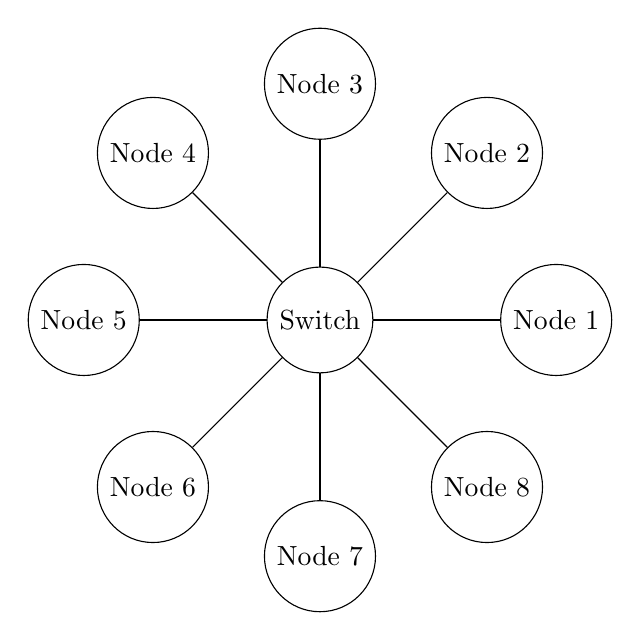
\begin{tikzpicture}
        % Number of nodes
        \def\numNodes{8}
        % Central node
        \node[draw, circle] (central) at (0,0) {Switch};

        % Calculate angle step based on the number of nodes
        \pgfmathsetmacro{\angleStep}{360/\numNodes}

        % Generate nodes in a circle
        \foreach \n in {1,...,\numNodes}{
            % Calculate angle for this node
            \pgfmathsetmacro{\angle}{\angleStep*(\n-1)}

            % Position node using polar coordinates
            \node[draw, circle] (Node\n) at (\angle:3cm) {Node \n};
          }

        % Draw connections between all nodes
        \foreach \i in {1,...,\numNodes}{
            \draw (Node\i) -- (central);
          }
      \end{tikzpicture}
    }
    \caption{Star Topology}
    \label{fig:star_top}
  \end{minipage}
  \hfill % Use \hfill to push the minipages to their respective sides
  % Start of the second minipage for the ring topology
  \begin{minipage}{0.3\textwidth}
    \centering
    \scalebox{0.6}{
      \begin{tikzpicture}
        % Number of nodes
        \def\numNodes{8}
        % Calculate angle step based on the number of nodes
        \pgfmathsetmacro{\angleStep}{360/\numNodes}

        % Generate nodes in a circle
        \foreach \n in {1,...,\numNodes}{
            % Calculate angle for this node
            \pgfmathsetmacro{\angle}{\angleStep*(\n-1)}

            % Position node using polar coordinates
            \node[draw, circle] (Node\n) at (\angle:3cm) {Node \n};

            % Connect each node to the next, creating a ring
            \pgfmathtruncatemacro{\nextNode}{mod(\n,\numNodes)+1}
            \draw (Node\n) -- (Node\nextNode);
          }
      \end{tikzpicture}
    }
    \caption{Ring Topology}
    \label{fig:ring}
  \end{minipage}
  \hfill % Use \hfill again for spacing
  % Start of the third minipage for the fully connected graph
  \begin{minipage}{0.3\textwidth}
    \centering
    \scalebox{0.6}{
      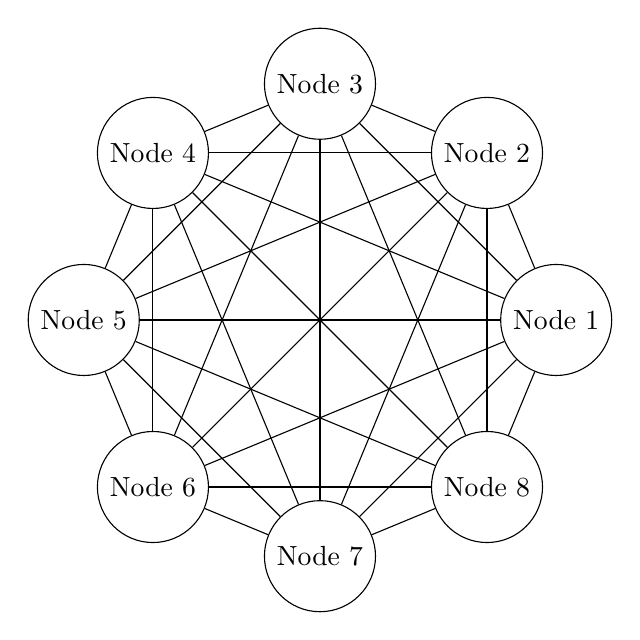
\begin{tikzpicture}
        % Number of nodes
        \def\numNodes{8}

        % Calculate angle step based on the number of nodes
        \pgfmathsetmacro{\angleStep}{360/\numNodes}

        % Generate nodes in a circle
        \foreach \n in {1,...,\numNodes}{
            % Calculate angle for this node
            \pgfmathsetmacro{\angle}{\angleStep*(\n-1)}

            % Position node using polar coordinates
            \node[draw, circle] (Node\n) at (\angle:3cm) {Node \n};
          }

        % Draw connections between all nodes
        \foreach \i in {1,...,\numNodes}{
            \foreach \j in {\i,...,\numNodes}{
                \ifnum\i=\j\relax
                  % Skip drawing a node to itself
                \else
                  \draw (Node\i) -- (Node\j);
                \fi
              }
          }
      \end{tikzpicture}
    }
    \caption{Connected Graph}
    \label{fig:fully_connected}
  \end{minipage}
  % End of the third minipage
\end{figure}


Next, the \textit{Ring Topology} depicted in figure \ref{fig:ring} is examined, where each node is connected to two other nodes,
forming a loop. This topology allows for a straightforward path of communication, with data traveling around the ring to reach its destination.
The diameter of this topology grows linearly with the number of nodes, making it less ideal as the network size increases.
% \todo{Note from Harumi: I swapped the following two sentences because I thought it read better that way given that the previous sentence gives a negative.}
On the plus side, the ring topology is relatively inexpensive to implement and scale, as adding more nodes simply involves creating two additional connections for each new node.
However, the bisection bandwidth of a ring topology is inherently limited, cutting the ring at any point to form two halves only requires severing two connections,
which could easily become a bottleneck in data-intensive applications.

Finally, the \textit{Fully Connected Network}, as shown in figure \ref{fig:fully_connected}, offers the most direct communication paths, with each node directly connected to every other node.
This topology boasts the lowest possible diameter of 1, as any two nodes can communicate directly without intermediary nodes.
The bisection bandwidth in this topology is maximized, given the sheer number of connections that would need to be severed to bisect the network.
However, the cost and complexity associated with a fully connected network are its most significant drawbacks.
The number of required connections grows quadratically with the addition of nodes, making this topology impractical for large-scale applications due to the prohibitive cost of implementing and maintaining such an extensive network.

In practice, most \ac{HPC} systems utilize a combination of these topologies, such as the \nameref{fig:fat_tree} (\ref{fig:fat_tree}) or \nameref{fig:hypercube}(\ref{fig:hypercube}), which strike a balance between performance, scalability, and cost\footcite{bestaHighPerformanceRoutingMultipathing2021b}.


\begin{figure}[!ht]

  \centering
  \vspace{0.5cm}
  \begin{minipage}{0.5\textwidth}
    \centering
    \scalebox{0.5}{
      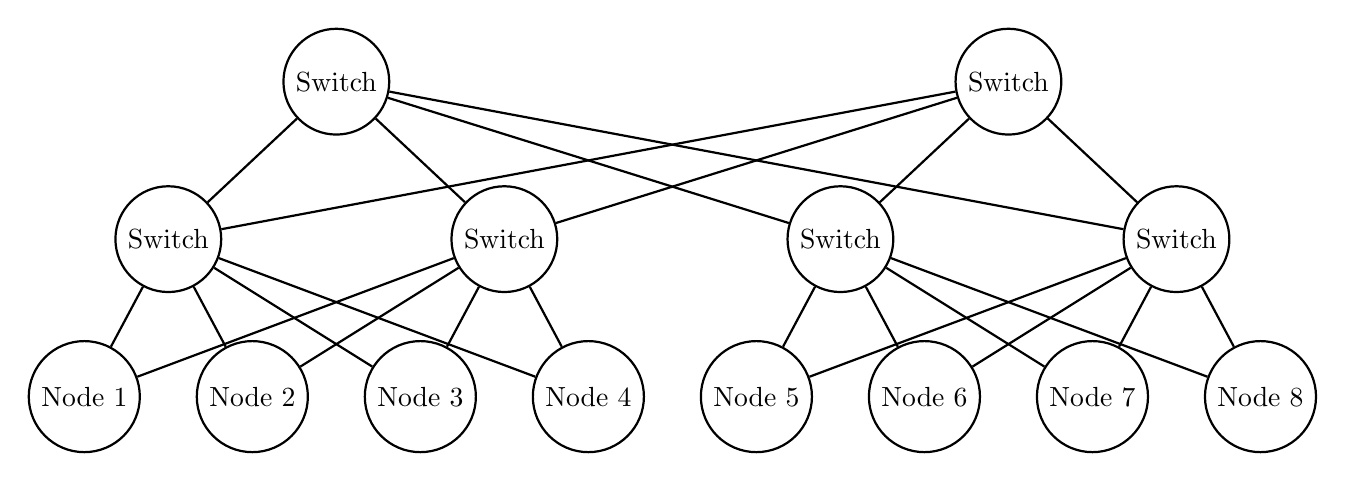
\begin{tikzpicture}[node distance={15mm}, thick, main/.style = {draw, circle}]
        \def\numNodes{8}
        \def\levelSep{2cm}
        \def\nodeSep{0.75mm}

        % Drawing the root switches 
        \pgfmathsetmacro{\nodesInRoot}{\numNodes/4}
        \foreach \i in {1,...,\nodesInRoot}{
            \pgfmathsetmacro{\xPos}{(\i - (\nodesInRoot+1)/2)*(4*\nodeSep)}
            \node[draw, circle] (root-\i) at (\xPos, 0) {Switch};
          }

        % Drawing the first level of switches
        \pgfmathsetmacro{\nodesInLevel}{\numNodes/2}
        \foreach \i in {1,...,\nodesInLevel}{
            \pgfmathsetmacro{\xPos}{(\i - (\nodesInLevel+1)/2)*(2*\nodeSep)}
            \node[draw, circle] (level1-\i) at (\xPos, -\levelSep) {Switch};
          }

        % Drawing the base nodes
        \foreach \i in {1,...,\numNodes}{
            \pgfmathsetmacro{\xPos}{(\i - (\numNodes+1)/2)*\nodeSep}
            \node[draw, circle] (base-\i) at (\xPos, -2*\levelSep) {Node \i};
          }

        % Connections
        % Root routers to each layer 1 router
        \foreach \root in {1,...,\nodesInRoot}{
            \foreach \lvlOne in {1,...,\nodesInLevel}{
                \draw (root-\root) -- (level1-\lvlOne);
              }
          }

        % Layer1 router 1 and 2 to nodes 1-4
        \foreach \i in {1,...,4}{
            \draw (level1-1) -- (base-\i);
            \draw (level1-2) -- (base-\i);
          }

        % Layer1 router 3 and 4 to nodes 4-8
        \foreach \i in {5,...,8}{
            \draw (level1-3) -- (base-\i);
            \draw (level1-4) -- (base-\i);
          }
      \end{tikzpicture}
    }
    \caption{Fat Tree Topology}
    \label{fig:fat_tree}
  \end{minipage}\hfill
  \begin{minipage}{0.5\textwidth}
    \centering
    \scalebox{0.5}{
      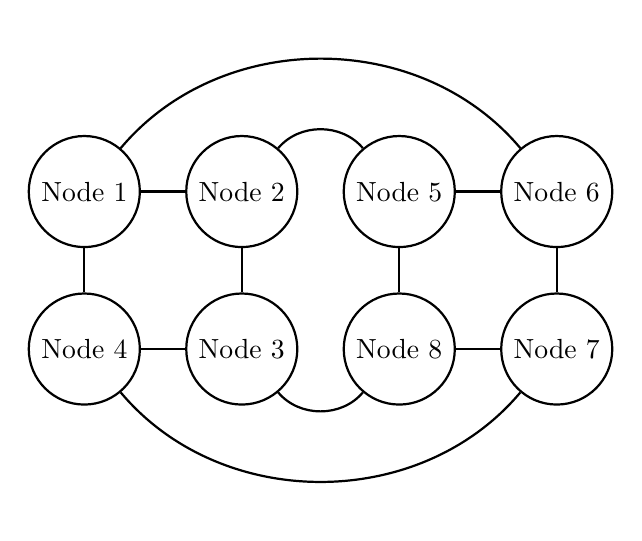
\begin{tikzpicture}[node distance={2cm}, thick, main/.style = {draw, circle}]
        % Nodes
        \node[main] (1)              {Node 1};
        \node[main] (2) [right of=1] {Node 2};
        \node[main] (3) [below of=2] {Node 3};
        \node[main] (4) [below of=1] {Node 4};
        \node[main] (5) [right of=2] {Node 5};
        \node[main] (6) [right of=5] {Node 6};
        \node[main] (7) [below of=6] {Node 7};
        \node[main] (8) [below of=5] {Node 8};

        % Connections
        \draw (1) -- (2);
        \draw (1) -- (4);
        \draw (2) -- (3);
        \draw (3) -- (4);
        \draw (1) edge[bend  left=50] (6); % Arching connection
        \draw (2) edge[bend  left=50] (5); % Arching connection
        \draw (3) edge[bend right=50] (8); % Arching connection
        \draw (4) edge[bend right=50] (7); % Arching connection
        \draw (5) -- (6);
        \draw (6) -- (7);
        \draw (7) -- (8);
        \draw (8) -- (5);
      \end{tikzpicture}
    }
    \caption{Hypercube Topology}
    \label{fig:hypercube}
  \end{minipage}
\end{figure}

% % \todo{should I use routing or switching? as IB uses switching and TCPIPoEthernet uses routing.  Note from Harumi: https://www.baeldung.com/cs/routing-vs-forwarding-vs-switching Routing is moving data between nodes; Switching is a subset of routing -- moving data from a node to multiple nodes. Are you asking about the figure? I think switch is correct there.}

% While there exist many more complex topologies, like \texttt{Dragonfly} or \texttt{Torus} topologies they 
% all trade off between the diameter, the bisection bandwidth and the cost according to the specific use case.


% % \footcite{eickhoffTopologyAwareWorkloadAnalyzer} also explains low diameter and high diversiyu topologies are important for HPC systems.
% % Explain the concepts of network topology and how different topologies (e.g., fat tree, torus, hypercube) impact performance.


% % % Storage Systems

% %     Elaborate on hierarchical storage management and the role of parallel file systems (e.g., GPFS, Lustre) in HPC.
% %     Address the challenges of I/O bottlenecks and how they can be mitigated.

\subsection{HPC Software Stack}

Now that we have discussed the hardware components and their configurations, we will dive into the software stack that powers \ac{HPC} systems.
While this is the only part we can directly interact with as developers, many of the decision made in the hardware stack have a direct impact on
the software we will be working with on the cluster.


\subsubsection{Operating Systems}
\label{sec:operating_systems}

% \todo{Note from Harumi: I heavily edited the following paragraph.}
% Haha Linux history is propably the most controversial part of the whole paper. :D
While the operating system is the most fundamental part of modern computers, in the context of \ac{HPC} systems there exists no competition to the Linux operating system,
which has had a 100\% market share in the \ac{HPC} Top500 list since 2017\footcite{top500OperatinststemsDevelopmentTime}.
Before its rise to dominance, Linux's competitors were its predecessors -- other, proprietary, UNIX-based operating systems that were
the default operating systems for most \ac{HPC} systems.
%But the \ac{HPC} community is complexly directed towards \gls{POSIX}-compliant systems\footcite{top500OperatinststemsDevelopmentTime}.
Linux has come to dominate the \ac{HPC} community for a number of reasons that include a desire to avoid vendor lock-in and licensing costs,
as well as an appreciation for the customizability and flexibility of Linux,
as its Kernel, Software and Libraries are all open source, which enables the community to optimize the system for their specific use case\footcite{rohitguptaLinuxOperatingSystem}.


\subsubsection{Programming Models}
\label{sec:programming_models}
As already mentioned above, the way the hardware works in \ac{HPC} systems is very closely tied into the way the software needs to be written.
This is especially true for this section, as the way the memory is distributed across the nodes and how the cores communicate with each other
,needs to be taken into account when writing the software, or at least assumed by the framework that is used.


\textbf{OpenMP}

OpenMP is a shared memory parallel programming model, it is the software counterpart of the \ac{SMP} hardware architecture, and works both with \ac{UMA} and \ac{NUMA} systems.
It is a set of compiler directives, library routines, and environment variables that enable the parallelization of code on shared memory systems \footcite{hermannsParallelProgrammingFortran}.
So it is designed to work on a single node of a given cluster, but able to utilize and combine the power ot the cores and memory of the whole node,
but cannot go beyond the boundaries of the node and communicate with other nodes\footcite{mitplasmascienceandfusioncenterIntroParallelProgramming2022}.
Compared to other parallel programming models, OpenMP presents a relatively high level of abstraction, being able to parallelize code with a few lines of code.
Its main advantage is its simplicity. OpenMP is based on compiler directives, which are added to the code and interpreted by the compiler to generate the parallelized code.
This makes it very easy to use, as the programmer does not need to worry about the specifics of the hardware as the compiler will take care of it\footcite{niklaswittmerParallelisierungMitOpenMP2018}.
While this is a great advantage for the programmer and lowers the barrier of entry for subject-matter experts of a specific field, it also has its drawbacks.
As the compiler makes relatively uninformed decisions about the parallelization, the performance of the parallelized code can be suboptimal\footcite{ruudvanderpasGettingOpenMPSpeed2014}.

It implements parallelization using a multithreaded fork-join model, where a single thread starts the program and then forks additional threads to run the parallelized code as can be seen in figure \ref{fig:fork_join} below.
So once a parallel region is defined by the programmer the process will fork the specified number of threads, which will run concurrently until the end of the region, where they join back together to continue the sequential execution of the code\footcite{laboratoryOpenMPProgrammingModel}.
While these threads are running concurrently, they have access to a shared memory space containing the previous linear state of the program,
but also have their own private memory space, which is used to store the variables that are only relevant to the specific thread\footcite{mitplasmascienceandfusioncenterIntroParallelProgramming2022}.

\begin{figure}[!ht]
  \centering
  \scalebox{0.8}{
    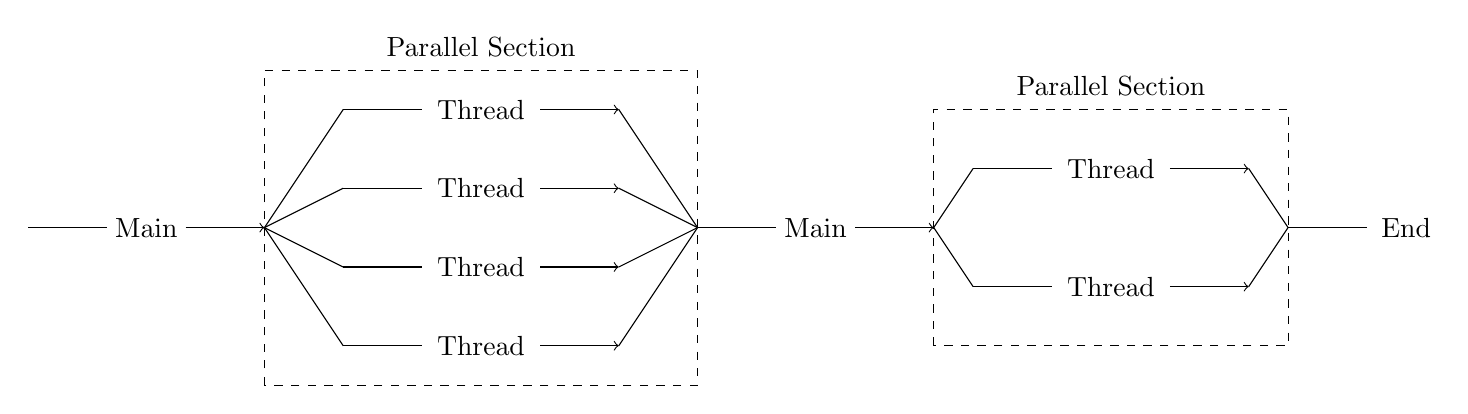
\begin{tikzpicture}[node distance=0.5cm and 1cm]
      % Main thread
      \draw (0,0) -- (1,0);
      \node at (1.5,0) {Main};
      \draw[->] (2,0) -- (3,0);
      % Linear Section Label

      % First Parallel Section Box
      \draw [black, dashed] (3,-2) rectangle (8.5,2);
      \node at (5.75,2.3) {Parallel Section};

      % Fork 1 x4 
      \foreach \y in {1.5, 0.5, -0.5, -1.5}{
          \draw (4,\y) -- (5,\y);
          % drawing connection to main 
          \draw (3,0) -- (4,\y);
          \node at (5.75,\y) {Thread};

          \draw[->] (6.5,\y) -- (7.5,\y);
          \draw (7.5,\y) -- (8.5,0);
        }

      \draw(8.5,0) -- (9.5,0);
      \node at (10,0) {Main};
      \draw[->] (10.5,0) -- (11.5,0);

      % Second Parallel Section Box
      \draw [black, dashed] (11.5,-1.5) rectangle (16,1.5);
      \node at (13.75,1.8) {Parallel Section};

      % fork 2 x2
      \foreach \y in {0.75, -0.75}{
          \draw (12,\y) -- (13,\y);
          % drawing connection to main 
          \draw (11.5,0) -- (12,\y);
          \node at (13.75,\y) {Thread};

          \draw[->] (14.5,\y) -- (15.5,\y);
          \draw (15.5,\y) -- (16,0);
        }

      \draw(16,0) -- (17,0);
      % draw end 
      \node at (17.5,0) {End};
      % Join Label

    \end{tikzpicture}
  }
  \caption{Fork-Join Model}
  \label{fig:fork_join}
\end{figure}
For example, a loop that would normally be executed sequentially can be parallelized with OpenMP
by adding the \texttt{\#pragma omp parallel for} directive in front of the loop.
This will tell the compiler to parallelize the loop, and the compiler will then generate the code to run the loop in parallel\footcite{mitplasmascienceandfusioncenterIntroParallelProgramming2022}.
On runtime instead of going through each iteration of the loop one by one,
all the iterations will be divided between the threads, which will then run the iterations concurrently.
The program then waits for all threads to finish before continuing.


\textbf{Message Passing}
\label{sec:message_passing}

If OpenMP is the standard for shared memory systems, then the \ac{MPI} is its equivalent for distributed memory systems.
It is a standardized and portable message-passing system designed to work on a wide variety of computers, and is language independent, supporting C, C++, and Fortran\footcite{groppUsingMPIPortable1999}.
In practical terms, \ac{MPI} serves as an \ac{API} that enables the inter-process communication across nodes and the network,
allowing the programmer to send and receive messages between the nodes, and to synchronize the processes\footcite{vishuvaishnavMessagePassingDistributed2023}.

While some implementations enable the use of shared memory within a node, which have become a valuable tool in hybrid systems,
\ac{MPI} itself is primarily designed around the actively sending and receiving messages
during runtime instead of accessing the memory directly.

\ac{MPI} is based on the \ac{SPMD} model, where each process runs the same program, but with different data, and can communicate with each other via messages.
This is done via the so-called \textit{rank} of the process, which is a unique \ac{ID} assigned to each process,
serving as an address for the process, used to send and receive the messages, without needing
to concern itself with the specifics of the underlying \gls{ISO/OSI model}\footcite{openmpiWhatOpenMPI2014}.

Messages in \ac{MPI} are sent and received either via point-to-point communication where the \textit{rank} of the sender and receiver are specified,
or via a collective communication, where information is sent or received from all or a subset of the processes\footcite{eickhoffTopologyAwareWorkloadAnalyzer}.
These collective operations can be split into two dimensions:

\begin{enumerate}
  \item \textbf{Data flow direction:} As a process can either send or request the reception of a message, the flow of communication can be either towards
        the initiating process, so a process might send a subtask to other processes(e.g. \textit{BROADCAST}) or request the results of a subtasks in order to continue(eg. \textit{GATHER})\footcite{dartmouthcollegeMPICollectiveCommunication}.
  \item \textbf{Data distribution:}
        The data a process sends/receives can either be a single value being replicated  across all processes (e.g. \textit{BROADCAST}) or a number of values being spread across the processes (eg. \textit{SCATTER})\footcite{dartmouthcollegeMPICollectiveCommunication}.
\end{enumerate}

% \todo{Maybe here I should add diagramm witht the different collective operations as matrixes like in the citation}

% The second important feature of \ac{MPI} is how and whether communication completeness is checked.
% As the default behavior of \ac{MPI} is to block until the message is send/received, the communication is inherently synchronous.
% This can leave some performance on the table, as the communication between the nodes is quite slow compared to the communication between the cores,
% therefore \ac{MPI} also provides non-blocking functions, which will return immediately, and the program can continue to run while the message is being send or received\footcite{shunyancheungAsynchronousCommunicationPrimitives}.

\textbf{Chapel/GASNet}
\label{sec:gasnet}

If OpenMP is the standard for shared memory systems, and \ac{MPI} is the standard for distributed memory systems, then Chapel is the standard for \ac{PGAS} systems.
Chapel is a high-level parallel programming language designed for productive parallel computing across a wide range of scales, from multi-core desktops to the supercomputers\footcite{chapel-lang.orgChapelOverview}.
Being based on the \ac{GASNet}, Chapel is able to work on both shared, distributed memory systems and hybrid systems, or even emulating multiple nodes on a \ac{SMP} system for development and testing\footcite{chapel-lang.orgMultilocaleChapelExecution}.
Making use of \ac{RDMA} in order to present a part of the memory as a large combined memory space, while in reality the memory is distributed across the nodes.
Being able to directly accessing the memory across the network, avoiding the overhead of the \ac{CPU} and the \ac{OS} in order to send and receive messages,
also has the advantage of being inherently asynchronous, as the memory can be directly accessed without needing to wait for the other process to be ready\footcite{dewanPavingWayDistributed2020}.

While some \ac{MPI} implementations such as \texttt{MVAPICH} or \texttt{OpenMPI} have started to implement \ac{RDMA} capabilities,
and \ac{GASNet} also supports network stacks which are not directly \ac{RDMA} capable,
each of these implementations was written with a specific use case in mind are oriented towards a specific use case.
An example for this is \ac{GASNet}s ability to access memory directly is not just limited to the \ac{CPU} memory,
but can also directly connect to auxiliary compute devices such as \ac{GPU}s in order to offload the
computations to the corresponding coprocessor\footcite{chamberlainPROGRAMMINGLANGUAGEPRODUCTIVE}.

\subsubsection{Workload Management Systems}

% \todo{Note from Harumi: are you allowed to write in the first person? I personally write "we" all the time, but I think this is the first time you have used it in this thesis.}
% So now that we have discussed how the hardware works on the nodes,
% Correction:
With an understanding of how the hardware works on the nodes,
how the cores can communicate with each other, even across the network,
and how these networks can be structured, the next step is to discuss
how when and where the code is being executed on the cluster.
This is where the workload management systems come into play, also known as schedulers or Batch systems,
as most of these systems main feature is the scheduler and primarily rely on a batch based distribution of jobs\footcite{hovestadtSchedulingHPCResource2003}.

The workload manager distributed jobs across the compute cluster.
Working with a list of computation tasks which are submitted by the users along with the
amount of resources they need, the workload manager is responsible for the distribution of the jobs across the cluster.
In order to optimize the utility of the cluster, the workload manager reduces the idle time of the nodes,
by fitting in as many jobs of different users as possible, trading off between quick execution and fairness\footcite{hpcwikiSchedulersHowToRunApplicationsonasupercomputer}.

One of the most common workload management systems is \ac{SLURM}, which is an open-source workload manager targeted towards \ac{HPC} systems\footcite{yooSLURMSimpleLinux2003}.
From the perspective of the user, \ac{SLURM} is a command line tool, which is used to submit jobs to the cluster
and from the perspective of the node it is a simple \gls{daemon} not to different from a remote shell\footcite{schedmdSlurmWorkloadManagera}.
But under the hood it is a highly complex system, checking the availability of the resources,
managing permissions and most importantly deciding the order of the jobs to be executed.
In its most basic form \ac{SLURM} is a \ac{FIFO} queue, where the jobs are executed in the order they are submitted,
which would lead to a low utilization of the cluster. Therefore, it does not strictly adhere to the \ac{FIFO} principle,
but slots in a lower priority job if it is able to run in a slot between regularly scheduled ones, as log as it does not delay any job of higher priority\footcite{schedmdSlurmWorkloadManagerb}

Additionally, \ac{SLURM} can be provided with information about the topology of the network,
supporting both torus and fat tree topologies, which can be used to optimize the placement of the jobs on the cluster,
by using an n-dimensional space filling curve in the former and a tree based algorithm in the latter in order to get the jobs
as close to each other as possible\footcite{schedmdSlurmWorkloadManagerc}.

\pagebreak